% ****************************************************************************************** % Dissertation template and document class
% Author  : 
% ****************************************************************************************** %
%%% For print copies
%% set 'singlespace' option to set entire thesis to single space, and define "\printmode" to remove all hyperlinks for printed copies of the thesis. Delete all output files before changing this mode -- it will turn hyperref package on and off
%\newcommand{\printmode}{}

%%% For the electronic copy, use doublespacing, define "\proquestmode" to use outlined links, instead of colored links. 
\documentclass[report,a4paper,12pt]{pieasthesis}
\newcommand{\proquestmode}{} %\printmode or \proquestmode
\title{AI Frameworks for Visual Traffic Surveillance, from Vehicle Classification to Event Detection}

\submitted{Januray 3, 2020}  % degree conferral date (January, April, June, September, or November)
\copyrightyear{2011}  % year in which the copyright is secured by publication of the dissertation.
\author{Assad Sultan \\ \& \\ Muneeb ur Rehman}
\adviser{Dr. Zulfiqar Hassan}  %replace with the full name of your adviser
%\departmentprefix{Program in}  % defaults to "Department of", but programs can change this.
\department{Electrical Engineering}
\degreeprefix{BS}
\degree{Electrical Engineering}
%%%%%%%%%%%%%%%%%%%%%%%%%%%%%%%%%%%%%%%%%%%%%%%%%%%%%%%%%%%%%\
    \renewcommand{\topfraction}{0.85}	% max fraction of floats at top
    \renewcommand{\bottomfraction}{0.6}	% max fraction of floats at bottom
    \setcounter{topnumber}{2}
    \setcounter{bottomnumber}{2}
    \setcounter{totalnumber}{4}     % 2 may work better
    \setcounter{dbltopnumber}{2}    % for 2-column pages
    \renewcommand{\dbltopfraction}{0.66}	% fit big float above 2-col. text
    \renewcommand{\textfraction}{0.15}	% allow minimal text w. figs
    %   Parameters for FLOAT pages (not text pages):
    \renewcommand{\floatpagefraction}{0.66}	% require fuller float pages
	% N.B.: floatpagefraction MUST be less than topfraction !!
    \renewcommand{\dblfloatpagefraction}{0.66}	% require fuller float pages
    

\usepackage{graphicx,verbatim,amsmath,multirow,longtable,booktabs,epsfig,epstopdf,multicol}
\setlength{\LTcapwidth}{\textwidth}
\usepackage[top=1in, bottom=1in, left=1.5in, right=1in]{geometry}
\usepackage[utf8]{inputenc}
\usepackage{float} 
\usepackage{fullpage}
\usepackage{pbox}

%%%%%%%%%%%%%%%%%%%%%%%%%%%%%%%%%%%%%%%%%%%%%%%%%%%%%%%%%%
%%% Printed vs. online formatting
\ifdefined\printmode
% Printed copy\usepackage{array}
\usepackage{makecell}

\renewcommand\theadfont{\normalsize\bfseries}
% url package understands urls (with proper line-breaks) without hyperlinking them
\usepackage{url}
\else
\ifdefined\proquestmode
\usepackage[hidelinks]{hyperref}
\hypersetup{bookmarksnumbered}
\makeatletter
\hypersetup{pdftitle=\@title,pdfauthor=\@author}
\makeatother

\else
\usepackage{hyperref}
\hypersetup{colorlinks,bookmarksnumbered}

% copy the already-set title and author to use in the pdf properties
\makeatletter
\hypersetup{pdftitle=\@title,pdfauthor=\@author}
\makeatother

% make the page number rather than the text be the link for ToC entries
%\hypersetup{linktocpage}
\fi % proquest or online formatting
\fi % printed or online formatting
\usepackage{sectsty}
\usepackage{lipsum}
\subsectionfont{\fontfamily{phv}\itshape\normalsize}
\subsubsectionfont{\normalsize}
\sectionfont{\large}
%\subsectionfont{\sffamily\itshape}
\setcounter{secnumdepth}{4} 
\setcounter{tocdepth}{4}
%%%%%%%%%%%%%%%%%%%%%%%%%%%%%%%%%%%%%%%%%%%%%%%%%%%%%%%%%%%%%\
%%%% Define commands

\newenvironment{indenttext}{
    \begin{list}{}{ \itemsep 0in \itemindent 0in
    \labelsep 0in \labelwidth 0in
    \listparindent 0in
    \topsep 0in \partopsep 0in \parskip 0in \parsep 0in
    \leftmargin 1em \rightmargin 0in
    \raggedright
    }
    \item
  }
  {\end{list}}

% another environment that's an indented list, with no spaces between items -- if we want multiple items/lines. Useful in tables. Use \item inside the environment.
% 	\raggedright makes them left aligned instead of justified
\newenvironment{indentlist}{
    \begin{list}{}{ \itemsep 0in \itemindent 0in
    \labelsep 0in \labelwidth 0in
    \listparindent 0in
    \topsep 0in \partopsep 0in \parskip 0in \parsep 0in
    \leftmargin 1em \rightmargin 0in
    \raggedright
    }

  }
  {\end{list}}
%%%%%%%%%%%%%%%%%%%%%%%%%%%%%%%%%%%%%%%%%%%%%%%%%%%%%%%%%%%%%\
%%%% Front-matter
% For early drafts, you may want to disable some of the frontmatter. Simply change this to "\ifodd 1" to do so.
\ifodd 0
% you can just skip the \acknowledgements and \dedication commands to leave out these sections.
\else
\dedication{Dedicated to our Parents for their love and affection}
% \acknowledgements{
% \input{front/acknowledgements}
% }
\abstract{

\chapter*{Abstract}
\addcontentsline{toc}{chapter}{Abstract}
\vspace{-3mm}
The key objective of this project is the detection \& classification of vehicles for traffic surveillance purposes.
Increasing accidents on roads have made the need of efficient methods to meet the detection \& classification
purposes significant. Several state of the art alogrithms exist which detect and classify the objects considering
some features but to acheive high precision in short time, we need robust algorithms. In the past few years, CNNs have
acheived a rapid success in accuracy and speed. In this project, a CNN based detector is used called as YOLO. The algorithm is
trained for a custom dataset. The still images are used for training made available using web scrapping to make a large dataset
to get good results during training. The dataset consists of vehicles of 5 different classes. After the classification 
mechanism, detection algorithms are used for the detection of objects in a still image 
and moving frames. 
\vspace{15mm}\ \\
\textit{Keywords: Deep Learning, Detection, Vehicles, Convolutional Neural Networks, Deep Neural Networks, YOLO}

}
%%%%%%%%%%%%%%%%%%%%%%%%%%%%%%%%%%%%%%%%%%%%%%%%%%%%%%%%%%%%%\
%%%% Hide some chapters

%%% If you want to produce a pdf that includes only certain chapters, specify them with includeonly, in addition to including all chapters below.
%\includeonly{ch-intro/chapter-intro}
%%% You can also specify multiple chapters.
%\includeonly{ch-intro/chapter-intro,ch-usage/chapter-usage}
%\includeonly{chap1,chap2,chap3}


%%%%%%%%%%%%%%%%%%%%%%%%%%%%%%%%%%%%%%%%%%%%%%%%%%%%%%%%%%%%%
%%%% Notes:

% Footnotes should be placed after punctuation.\footnote{place here.}
% Generally, place citations before the period~\cite{anotherauthor}.
% The proper usage for i.e., and e.g., include commas ``(e.g., option A, option B)''
%%%%%%%%%%%%%%%%%%%%%%%%%%%%%%%%%%%%%%%%%%%%%%%%%%%%%%%%%%%%%
%%%% Import chapters
\usepackage{fancyhdr}
\usepackage{graphicx}
\usepackage{caption}
\usepackage{subcaption}
\usepackage{xcolor}
\usepackage{minted}

\setminted{fontsize=\footnotesize}

\fancypagestyle{plain}{
\fancyhf{} % clear all header and footer fields 
\fancyhead[R]{\thepage} %RO=right odd, RE=right even

\renewcommand{\headrulewidth}{0pt} 
\renewcommand{\footrulewidth}{0pt}} 
\usepackage[titletoc]{appendix}
\definecolor{bg}{rgb}{0.95,0.95,0.95}
\newenvironment{longlisting}{\captionsetup{type=listing}}{}
\begin{document}

\makefrontmatter

\chapter{Introduction}
\label{1}
\section{Motivation}

With the development of science and technology, there may arise crucial 
problems. Rising traffic in the country gives birth to rising accidents. To 
avoid/minimize the accidents, proper surveillance is required. Detection 
and tracking of vehicles have become a key component in traffic 
surveillance and automatic driving. Traditional algorithms like Gaussian 
Mixed Model (GMM) has achieved encouraging success in this field \cite{chap_1_article:1}. But due 
to variation in illumination, occlusion, background clutter etc. detection 
of vehicles is still a challenge. 
Deep Neural Networks (DNNs) have gained a lot of attention in 
past few years. Due to the betterment of deep learning, object 
detection has achieved major advancements in recent years. The work 
in this project is based on DNNs to detect and classify vehicles from 
a dataset collected from images and videos.

\section{Background}

Classical methods of vehicle detection were based on some 
sort of features like symmetry, edges, texture, underbody shadows 
and corners \cite{chap_1_article:2}. These methods were easy to describe and perform 
in specific kind of applications. These methods fail in many situations 
like due to less illumination of highway. With the advent of 
deep learning, a subset of machine learning, the detection and 
classification mechanism have dramatically improved. Machine learning 
and deep learning are sub-branches of computer intelligence which help 
in the process of vehicle classification to event detection. 
Using deep learing techniques, we are going to focus on a specific kind 
of detection (deep learning has grown its branches in almost every 
kind of image recongnition, text recognition, face detection etc), vehicle 
detection. Using deep learning based Convolutional Neural Networks (CNNs) 
which is a wide field for object detection, classification, sementic 
segmenation etc. These networks take input images, learn features, adjust 
weights and then detect the targets from test data. In deep learning, 
algorithms automatically learn features unlike machine 
learning algorithms, we have to pass features to train the 
model. Our work is based on Deep Neural Networks (DNNs).

\section{Goals \& Objectives}

The goal of this project is to make a deep learning based model (using Python) for vehicle detection and classification. Main objectives are summarized as:
\begin{itemize}
\item Collection of datasets (images dataset of car, truck classes etc. and videos).
\item Design of Convolutional Neural Network
\item Configuration of training options (AlexNet, VGGNet, ResNet etc.)
\item Training of detector (RCNN, Fast- RCNN, Faster-RCNN, YOLO etc.)
\item Evaluation of the trained detector
\end{itemize}

\section{Challenges}

Human can understand and interpret images in a 
second or less. For machines, it is not easy to achieve 
accurate results unless models are trained properly. Firstly, proper 
training is a challenging task for a customized data. Detection 
algorithms are also hard to implement as we must have recommended 
GPU requirements and best choice of algorithm for good results. Videos 
which are moving frames, it is difficult to draw accurate bounding boxes 
in a video having say 30 frames per second 
means 30 images are splashed in a second. 	


\section{Organization of Thesis}

\textbf{Chapter \ref{Chapter 2}}: Chapter 2 is about literature review. It is about
the whole reading and understanding of Image classification \& detection.

\noindent\textbf{Chapter \ref{Chapter 3}}: This chapter is about Convolutional Neural Networks. All CNN architectures with their details
are discussed.

\noindent\textbf{Chapter \ref{Chapter 4}}: This chapter contains all
the procedural details of the dataset formation for classifier,
training process and evaluation of results along with all the relevant codes.

\noindent\textbf{Chapter \ref{Chapter 3}}: This chapter deals with\
the training and testing of a YOLO based cutom object detector.
All the relavant codes and results are attached for easy understanding.

\chapter{Literature Review}
\label{Chapter 2}

\section{History of Object Recognition \& Detection}

The field of computer vision deals with how the computers can be made to understand digital images or videos. 
The history of Computer Vision can be traced back to 1960s. Before that people had tried for alphabet recognition 
but those attempts had not led very far. L.G. Roberts, in his Ph.D thesis mentioned about the perception 
of solid objects. Using the properties of three dimensional transformations and the laws of nature, a procedure 
was developed which had been able to identify objects as well as determine their orientation and position in space \cite{chap_2_article:1}. 

In 1970s, David Marr wrote a book on visual recognition. In his book he mentioned that in order to take an 
image and to arrive at a final holistic full 3D representation of the visual world, we must go through 
several processes. The first process he calls is “Primal sketch” where edges, bars, ends and virtual lines 
are determined. Next is “two and half-D sketch” leading to “3-D sketch”  \cite{chap_2_article:2}. Another very important seminal 
group of work happened in 1970s when people began to ask the question, “how can we move beyond simple block 
world and start recognizing real objects?” Two group of scientists proposed similar ideas, one 
is called “generalized structure” and other is called “pictorial structure”. The basic idea was that 
every object is composed of simple geometric primitives \cite{chap_2_article:3}. 

In 80s, David Lowe tried to recognize razors by constructing lines and edges and mostly straight lines 
and their combination. At those times, it was very hard to solve an image recognition problem due to 
limited resources. From 1999 to 2000, statistical machine learning techniques started to gain momentum. Such 
techniques are support vector machines, boosting, graphical models etc. In 2006, FujiFilm rolled out first 
digital camera with face detection feature.

One of the very influential way of thinking in the late 90s till the first 10 years of 21st century was feature 
based recognition. An important work was done by David Lowe based on a feature called as SIFT feature. The idea 
was that to match one stop sign shown in Figure \ref{fig:2.1} with another stop sign is very difficult, because there might 
be all kinds of changes due to camera angles, occlusion, viewpoint, lighting and just the intrinsic variation of 
the object itself. Despite it is inspired to observe that there are some parts of the object that tend to remain 
unchanged. So, the task of object recognition began with identifying those features on the object and match these 
features to a similar object \cite{chap_2_article:4}.

\begin{figure}[t]
	\centering
	\includegraphics[width=0.80\textwidth]{CHAPTERS/Chapter-2/Images/2.1.png}
	\caption{SIFT \& Object Recognition}
	\label{fig:2.1}
\end{figure}
In 2009, the ILSVRC was 
rolled out. This data set contains 1.4 million images of different classes. In 2012, the 
error rate was dropped to almost 16 \% \cite{chap_2_article:5}. The winning algorithm was based on 
CNNs. This work was published in 2012 introducing AlexNet, which brought a tremendous change in the field of image recognition. This thesis is based on image 
classification and detection using CNNs. 

\section{Basics of an Image}
To start with, we must understand all about an image, the information of 
an image that is important to a machine. A digital image is an information of a picture 
encoded in a digital form. It consists of pixels. The number of pixels 
in is the spatial resolution of an imahge, which 
relates to the image quality. The higher the spatial resolution, the better 
is the image quality. The resolution of an image is normally denoted by width $\times$ height. 
The numbers of bits used in encoding each pixel level also affects the image quality \cite{chap_2_article:6,chap_2_article:7}. 

\subsection{8-Bit Gray Level Images}
Images encoded on a gray scale ranging from 0 to 255 are called as
8-bit gray level images. The number 0 represents full black
and 255 represents a full white. The numbers in between 
represent the shades of gray. For example, for a 640 $\times$ 480 bit 
image, we need 307.2 kilobytes to store it. Figure \ref{fig:2.2} shows a 
grayscale image format. The pixel value indicated 
in the box has a value of 25 in 8-bit format. 

\begin{figure}[H]
	\centering
	\includegraphics[scale = 0.5]{CHAPTERS/Chapter-2/Images/2.2.png}
	\caption{Grayscale Image format}
	\label{fig:2.2}
\end{figure}

\subsection{2.2	24-bit Color Images}
Each pixel of an image in a 24-bit color images is 
encoded with Red (R), Green (G) and Blue (B) values. Each component of a 24-bit
images is encoded in 8 bits. Thus we get a total of 24 bits for a
a complete color RGB image. Having 
such an image, we have $2^{24} = 16.777216 \times 10^{6} \approx 16\:M$ colors.
As an example, take an image of resolution 640 $\times$ 480 in 24-bit color 
representation, it will require 922 kilobytes storage memoey.
Figure \ref{fig:2.3} shows the format for the 24-bit 
color image where the indicated pixel has 8-bit RGB components.

\begin{figure}[H]
	\centering
	\includegraphics[width=0.80\textwidth]{CHAPTERS/Chapter-2/Images/2.3.png}
	\caption{The 24-bit color image and its RGB components}
	\label{fig:2.3}
\end{figure}

\subsection{8-Bit Color Images}
Another popular format of images is an 8-bit color image. The pixel 
values are indexed from 0 to 255. Each index represents an entry of the 
color map. These images are called color indexed images. As an example, figure 2.4 shows 
a color indexed image having a pixel value of 5, which is the index for the entry of 
the color table. There are 3 color components having 
RGB values of 66, 132 and 134 respectively. 
Each component is encoded in 8 bits. There are 
only 256 different colors in the image. For instance, a
$640\times 480$ 8-bit color image requires 307 kB memory
for storage and 768 bytes (3 $\times$ 256) for storing
color map.

\begin{figure}[H]
	\centering
	\includegraphics[width=0.80\textwidth]{CHAPTERS/Chapter-2/Images/2.4.png}
	\caption{The 8-bit color indexed image}
	\label{fig:2.4}
\end{figure}

\subsection{Intensity Images}
In section 2.1, we mentioned that a grayscale image uses a 
pixel value in the range 0-255. A 0 value represents black while 255 
represents white. In some processing environments, floating point representations 
are used. The grayscale image has an intensity value normalized from 0 to 1, where 0 is 
for black and 1 is for white. In Figure 2.5, we have a grayscale intensity 
image, where the specfied pixel shows 0.5988 intensity value.

\begin{figure}[H]
	\centering
	\includegraphics[scale = 0.75]{CHAPTERS/Chapter-2/Images/2.5.png}
	\caption{The grayscale intensity image format}
	\label{fig:2.5}
\end{figure}

\subsection{Red, Green, and Blue Components and Grayscale Conversion}

For processing applications, we often need conversion from an RGB image to grayscale. There are two popular methods, one is average method where a grayscale value is obtained by just averaging the red, green and blue pixel values. The other is luminosity method, where we use approximately 30 \% of Red, 59 \% of Green and
11\% of Blue to form a grayscale image.
\begin{equation}
	\mbox{New grayscale image} = 0.3R + 0.587G + 0.114B
\end{equation}
\section{Image Classification}
Humans can understand and depicts the information contained in an image. On the other 
hand, machines cannot identify the image and retrieve information from it on its own. To 
achieve that purpose, we make the machines learn from examples and when it has learned 
enough, it may extract information from an image from an outside world and recognize it.

There exist many algorithms for image classification. One of them is BoW 
model, which is common for document classification and natural language 
processing. In addition to document classification, the BoW model can also be used for 
image classification. We extract a set of features from an image and count 
their occurrence. We have different algorithms for feature extraction. For example, in 
BoW model, SURF algorithm was used \cite{chap_2_article:8}. Other interesting image 
classification methods include texture analysis. However, a gain in performance has been 
brought by using neural networks. With the introduction of AlexNet architecture in 
2012, the error rate was dropped tremendously. Due to robustness of these 
algorithms, the CNNs are widely used for 
image recognition and classification nowadays. 

The problem of image classification can be stated as: \textit{“Given a set of 
images labeled with a single category, the machine has to predict a new set 
of images by assigning it a label and test the accuracy of the predictions”}. For 
example, in Figure \ref{fig:2.6} an image classification model takes a single image
as an input and allocates probabilities to 4 labels, {cat, hat, dog, mug}.
The computer sees the image as a 
3D-array of numbers. The cat example image is 248 pixels wide and 400 pixels in height 
with three color channels, Red, Blue and Green, therefore, a total 
of 248 $\times$ 400 $\times$ 3  = 297,600 numbers. Each number is an integer with values 
in range 0-255. What our task is to extract out of these 
thousands of numbers, a single label, such as “cat”. 

\begin{figure}[H]
	\centering
	\captionsetup{justification=centering,margin=2cm}
	\includegraphics[width=0.80\textwidth]{CHAPTERS/Chapter-2/Images/2.6.png}
	\caption{A 3D-array of numbers from 0 to 255 of size width $\times$ height $\times$ 3. 3 represents color channels}
	\label{fig:2.6}
\end{figure}

There are a multiple challenges linked with this. There 
may exist viewpoint variation, scale variation, deformation, occlusion (a small portion 
of object is displaying), background clutter, illumination conditions and intraclass 
variations. How do we end up writing an algorithm for image classification? Researchers have 
arrived at the point that in order to solve this problem, use data-driven approach. Instead 
of writing a code to specify everyone categories of interest look like, we provide computer 
many examples of images of each class and then develop the algorithm that look at these 
examples and learn about the visual representation of each class. This approach is known 
as data-driven approach. So, the image classification pipeline can be summarized as:

\begin{itemize}
\item Input of the system is a training dataset composed 
of N images of labeled with K different classes.
\item Using this training set, we train a classifier to learn how do these classes look like.
\item After that, test this classifier on a new dataset and then compare the results with the true labels of the images.
\end{itemize}

\subsection{Convolutional Neural Networks}

CNNs are the most famous network used 
for classification problems of images. The idea behind CNNs is that a 
understanding of an image locally is good enough. A practical advantage is 
that if we have less parameters, it will reduce the amount of data to train 
a model and improves the time of learning. A CNN has weights to look at a small 
patch of image. 

A convolution is a weighted sum of  the pixel values of an image, as 
we have a sliding window moving across the whole image. It gives another 
image having the same size. A CNN typically consists of 3 layers:

\begin{enumerate}
	\item Convolution Layer
	\item Pooling Layer
	\item Fully Connected Layer

\end{enumerate}
There are some batch normalization layers in some old CNNs 
but not used these days. (Details of CNNs are covered in chapter 3).

\subsubsection{CNN Architectures}
As mentioned before, the ImageNet project is an enormous visual database cretaed for research purposes. This 
project runs on an yearly contest named as ILSVRC, where different algorithms take 
part in competitions to classify and detect objects. Here 
we will talk about the competition top competitors \cite{chap_2_article:9}.
\begin{itemize}
	\item LeNet-5 (1998)
	\item AlexNet (2012)
	\item ZFNet (2013)
	\item GoogleNet (2014)
	\item VGGNet (2014)
	\item ResNet (2015)
\end{itemize}
\paragraph*{LeNet}

It is a 7-layer convolutional network by 
Yann LeCun et al. in 1998. It is used to classify digits and was applied by 
several banks to recognize handwritten numbers on cheques. The processing 
of higher resolution images need more convolutional layers, so this 
technique is restricted to the availability of resources \cite{chap_2_article:10}.

\begin{figure}[H]
	\centering
	\captionsetup{justification=centering,margin=2cm}
	\includegraphics[scale= 0.8]{CHAPTERS/Chapter-2/Images/2.7.jpg}
	\caption{Architecture of LeNet-5, original image published in [LeCun et al., 1998]}
	\label{fig:2.7}
\end{figure}


\paragraph*{AlexNet (2012):}
In 2012, Krizhevsky et al. introduced AlexNet which 
outperformed all the prior competitors and won the challenge 
by reducing the error to 15.3 \%.  This network had a similar architecture 
like LeNet but was deeper with more filters per layer. It 
consists of 11 layers between input and output. 

 
\begin{figure}[H]
	\centering
	\captionsetup{justification=centering,margin=2cm}
	\includegraphics[scale = 0.6]{CHAPTERS/Chapter-2/Images/2.8.jpg}
	\caption{An illustration of the architecture of AlexNet CNN}
	\label{fig:2.8}
\end{figure}

\paragraph*{ZFNet (2013):}
This architecture was the winner of 2013 ILSVRC. It achieved 
an error rate of 14.8 \%. It was achieved by tweaking the 
hyperparameters of AlexNet while maintaining the same structure and 
adding deep learning elements \cite{chap_2_article:11}. The architecture 
is shown in \ref{fig:2.9}.

\begin{figure}[H]
	\centering
	\captionsetup{justification=centering,margin=2cm}
	\includegraphics[scale = 0.6]{CHAPTERS/Chapter-2/Images/2.9.jpg}
	\caption{Architecture of 8 layer ZFNet Model}
	\label{fig:2.9}
\end{figure}

\paragraph*{GoogleNet (2014):}
This architecture was the winner of  ILSVRC, 2014. It achieved a top-5 
error rate of 6.67 \%. It was close to human level performance. The network 
was inspired by LeNet but implemented a new element which is dubbed an 
inception module. It used batch normalization, image distortions and RMSprop. This architecture consists of 22 layers but a 
reduced number of parameters from 60 million to 4 million \cite{chap_2_article:12}. 

\paragraph*{VGGNet (2014):}
The VGGNet was developed by Simonyan and Zisserman. It was 
runner-up in ILSVRC, 2014. It consists of 16 convolutional 
layers and popular because of its uniform architecture. A challenging thing in 
VGGNet is that it consists of 138 million parameters \cite{chap_2_article:13}.
\begin{figure}[H]
	\centering
	\captionsetup{justification=centering,margin=2cm}
	\includegraphics[scale = 0.6]{CHAPTERS/Chapter-2/Images/2.11.png}
	\caption{An illustration of the architecture of VGGNet CNN}
	\label{fig:2.10}
\end{figure}

\paragraph*{ResNet (2015):}
In 2015, Residual Neural Network (ResNet) by Kaiming He et al. was introduced. It was a new
architecture with “skip connections” and features heavy batch normalization. These connections are known as gated units. There are 152 layers but still less complex than VGGNet. It achieved a top-5 
error rate of 3.57 \% which beats human-level performance \cite{chap_2_article:14}. 

\begin{figure}[H]
	\centering
	\captionsetup{justification=centering,margin=2cm}
	\includegraphics[width = 0.8\textwidth]{CHAPTERS/Chapter-2/Images/2.12.png}
	\caption{ResNet Architecture}
	\label{fig:2.11}
\end{figure}

AlexNet has parallel two CNN line trained on two GPUs with cross-connections, GoogleNet has 
inception modules, ResNet has residual connections.

\subsubsection*{Summary Table}
\begin{table}[H]
	\caption{Comparison of Different CNN Architectures}
	  \begin{center}
		\scalebox{.85}
		{\begin{tabular}{|l |l |l |l |l |}
		\hline
		Year & CNN & Developed by & Top-5 error rate (\%) & No. of Parameters \\ \hline
		1998  & LeNet(8) & Yann LeCun et al. &  &  60 thousand 
		\\ \hline
		2012  & AlexNet(7) & Alex Krizhevsky et al. & 60 million &
		\\ \hline
		2013   & ZFNet() &  Mathhew, Zeiler \& Rob Fergus & 9 &
		\\ \hline %
		2014 & GoogleNet(19) & Google & 6.67  & 4 million
		\\ \hline
		2014 & VGGNet(16) & Simonyan, Zisserman & 7.3 & 138 million
		\\ \hline
		2015 & ResNet(152)& Kaiming He & 3.6 & 
		\\ \hline   
		\end{tabular}}
	  \end{center}
\end{table}

We have discussed tha basics of an image, classification and famous models used
for classification purposes. The other part of the project deals with
the detection algorithm which is discussed in detail in chapter \ref{Chapter 5}.
In next chapter we will explore about CNNs and we will continue our discussion
of classifier in chapter \ref{Chapter 4} starting with dataset leading to the
results in detail. The models discussed will not be used as they are. 
Cutomised model according to the nature of the dataset and need will be used.
We will solve two class problem at first and having the results noted, 
we will train a classifier for five classes.


\chapter{Convolutional Neural Networks (CNNs)}
\label{Chapter 3}

CNNs are types of artificial neural networks used 
for object detection and image classification etc. Neural Networks 
are brain-inspired set of algorithms that are expected to mimic the working 
of human brain. Billions of neurons in our brain process information through 
electrical signals. Dendrites receive external information or stimuli in form of 
electrical impulses which is further processed in the cell body where it integrates 
all the signals coming in and the output is carried away to the downstream neurons 
through Axons \cite{chap_3_article:1}. The neuron chooses to either reject or accept the signal depending on the signal strength. Likewise, an artificial neural network has large  number of interconnected nodes called as neurons. The computational node and cell body of neuron works in kind of a similar way where we have large number of signals coming as inputs to neuron. Each signal has a weight W associated with it and the 
summation of these weighted inputs is passed to the activation function where 
 non-linearity is introduced in the output. Neural networks have the ability to gradually 
update the weights of the interconnections of the neuron until desirable results 
are obtained during the training phase of network.

\begin{figure}[H]
	\centering
		\includegraphics[width=0.70\textwidth]{CHAPTERS/Chapter-3/Images/3_1.jpg}
	\caption{Working of a single computational node}
	\label{fig:3.1}
\end{figure}

These neurons or computational nodes are organized 
into layer where there are highly interconnected to the neurons 
of following layer. The input layer of the feed forward neural 
networks feeds the information to the network and no kind of mathematical 
computation is performed. The hidden layer also known as distillation layer 
acts like a cell body and performs computation to extract salient features and 
patterns from the input data. Figure \ref{fig:3.2} a simple 
feed forward neural network having one 
hidden layer \cite{chap_3_article:2}.
The output layer simply provides the results for given information. 

\begin{figure}[H]
	\centering
		\includegraphics[width=0.70\textwidth]{CHAPTERS/Chapter-3/Images/3.2.png}
	\caption{Simple Feed Forward Neural Network with one hidden layer}
	\label{fig:3.2}
\end{figure}

The pixels of the image are arranged in a particular 
way i.e. the appearance of the picture will be changed 
if we change the coordinate of one pixel. However, simple feed 
forward neural network loses to learn the inherent spatial 
relationships within images and fails to extract high level features 
needed for image classification. CNNs are types 
of neural networks that learn visual filters to recognize higher level 
image features and the spatial information is preserved. As a result, you 
end up learning this hierarchy of filters where filters at the early stage 
usually represents low level features like edge detection, gradient orientation 
and learning more and more complex features in the later stages.

\section{Convolutional Neural Networks Architecture}

There are three types of layers associated with CNN. These layers include convolutional layers, pooling layers and fully connected layers.When we stack together these layers, we get a CNN architecture. A general
architecture of CNNs with two convolutional layers is shown in \ref{fig:3.3} \cite{chap_3_article:2}.

\begin{figure}[H]
	\centering
		\includegraphics[width=0.80\textwidth]{CHAPTERS/Chapter-3/Images/3.3}
	\caption{Convolutional Neural Network Architecture with two convolutional layers}
	\label{fig:3.3}
\end{figure}

\subsection{Convolutional Layer}
Convolutional layers are integral part of CNNs and when these layers are stacked
together, we start extracting more simple 
features and then aggregating these into more complex features later 
on. There is a set of learnable filters also called as kernels whose
height and width are smaller than the input image and always extend 
to the full depth of the input volume. We slide the filter over entire 
image to perform the operation of convolution i.e. multiplying each element of input image with the feature detector. The resultants are 
summed up and the value is assigned to the top left corner of receptive field 
as shown in figure 3.4 \cite{chap_3_article:4}.

\begin{figure}[H]
	\centering
		\includegraphics[width=0.70\textwidth]{CHAPTERS/Chapter-3/Images/3.4}
	\caption{3x3 filter with stride value of 1}
	\label{fig:3.4}
\end{figure}

The kernel window slides right or downward by a 
certain value known as stride value in each step and we repeat the process
whole image is processed. Stride value of
1 moves the filter 1 pixel in each step. This results in a feature map with 
much smaller size than the input image and keeps on shrinking at every layer 
which is usually not desirable. Thus, dimensionality of the input image can be 
preserved by padding zero-pixel values across every side of image.

\begin{figure}[H]
	\centering
		\includegraphics[width=0.70\textwidth]{CHAPTERS/Chapter-3/Images/3.5}
	\caption{Result  of 3x3 filter of Stride 1 with padding}
	\label{fig:3.5}
\end{figure}

In reality, we apply multiple filters to the same 
input image and feature maps are obtained depending upon the 
number of filters. In this case the output of convolutional layer 
is represented with a 3D matrix with dimensions of height, width 
and depth, where depth 
shows the no. of filters applied on the image. 

\begin{figure}[H]
	\centering
		\includegraphics[width=0.70\textwidth]{CHAPTERS/Chapter-3/Images/3.6}
	\caption{Multiple filters applied on one input}
	\label{fig:3.6}
\end{figure}

\subsubsection{Activation Functions}

It is like mathematical function that we apply to every neuron present in the network and it decides that whether to activate the neuron 
or not depending on how much neuron’s input is relevant to model’s prediction. 
In this way, a non-linearity is introduced in the output with the help of activation function. Without activation function, our network will be reduced to a simple 
regression model which would be unable to model and learn complex and complicated 
form of data. Thus, non-linear functions make neural networks capable 
of performing non-linear transformations to learn complex kinds of data such 
as 	images, videos etc. A good activation 
function should have the following properties:
\begin{itemize}
\item It should be zero centered because when back propagating gradient descent, the resulting values of gradient will either be all positive or all negative. Thus, it will affect the gradient based optimization process as we can only follow zig-zag path to reach the optimal point.
\item It shouldn’t kill the gradient flow i.e. neurons get saturated on the boundaries of activation and local gradient comes out to be zero. As a result, it nullifies the gradient flow during back propagation and dead neurons will stop updating.
\item It should be computationally efficient as activation function will be computed across millions of neurons for each input. Moreover, back propagation technique also puts constraint on the choice of activation function i.e. it should be differentiable.

\end{itemize}

\paragraph*{Sigmoid Function:}
A sigmoid function can be represented by the mathematical function:
\begin{equation}
	sig(z) = \frac{1}{1+e^{-z}}
\end{equation}
This function takes input a real value and squeezes 
it between 0 and -1 i.e. very large values. It is often called
as squashing function as the large negative and positive 
values becomes 0 and 1 respectively \cite{chap_3_article:5} . But the sigmoid function 
output is not zero-centered, and it also kills the neurons as function 
gets saturated at higher values. That’s why sigmoid function are usually 
not preferred in neural networks because of these drawbacks.

\begin{figure}[H]
	\centering
		\includegraphics[width=0.70\textwidth]{CHAPTERS/Chapter-3/Images/3.7.jpg}
	\caption{Sigmoid Function}
	\label{fig:3.7}
\end{figure}
\paragraph*{Tanh Function:}
A tanh sigmoid function can be represented by the following mathematical function:
\begin{equation}
	tanh(z) = \frac{e^{z}-e^{-z}}{e^{z}+e^{-z}}
\end{equation}

It takes the real input value and squashed it between -1 and 1 i.e. very 
large negative and positive values are mapped into -1 and 1 respectively \cite{chap_3_article:5}. As 
a result, this non-linear activation function gives zero-mean data, but it 
still gets saturated at higher values as shown in \ref{fig:3.8}. However, tanh 
activations functions are preferred over sigmoid functions in neural networks.

\begin{figure}[H]
	\centering
		\includegraphics[width=0.70\textwidth]{CHAPTERS/Chapter-3/Images/3.8.jpg}
	\caption{Tanh function}
	\label{fig:3.8}
\end{figure}

\paragraph*{ReLU Function:}
ReLU stands for Rectified Linear unit and is represented by the following equation:

\begin{equation}
	ReLU(z) = max(0,z)
\end{equation}

It takes real values as an input and sets all the negative 
values equal to zero \cite{chap_3_article:3}. It is computationally very efficient as no 
complicated math need to be performed. And it is the most frequently used 
activation function in neural networks as it increases the convergence rate 
of gradient descent by six times as compared to sigmoid and tanh activation 
functions. However, the function doesn’t get saturated for larger values of 
inputs, but the neurons often stuck in a negative side giving zero local gradient 
and neuron will never get a chance to update in gradient descent learning process. 
This problem is also known as dying ReLU and it often occurs due to high learning 
rate or there is a large negative bias. Leaky ReLU can be used to avoid this 
situation. Leaky ReLU is very similar to original ReLU and the only difference 
is that now instead of being flat in the negative regime, we are going to give 
slight negative slope here. This solves a lot of problems we mentioned earlier
as it doesn’t saturate in the negative space and still very computationally efficient \cite{chap_3_article:3}.

% \begin{figure}
% 	\centering
% 	\begin{subfigure}{.5\textwidth}
% 	  \centering
% 	  \includegraphics[width=.4\linewidth]{CHAPTERS/Chapter-3/Images/3.9a}
% 	  \caption{A subfigure}
% 	  \label{fig:3.9(a)}
% 	\end{subfigure}%
% 	\begin{subfigure}{.5\textwidth}
% 	  \centering
% 	  \includegraphics[width=.4\linewidth]{CHAPTERS/Chapter-3/Images/3.9b}
% 	  \caption{A subfigure}
% 	  \label{fig:3.9(b)}
% 	\end{subfigure}
% 	\caption{ReLU and Leaky ReLU Function}
% 	\label{fig:test}
% \end{figure}

\begin{figure}%
    \centering
    \subfloat[\label{fig:3.9(a)}]{{\includegraphics[height = 4.38cm, width=5cm]{CHAPTERS/Chapter-3/Images/3.9a} }}%
    \qquad
    \subfloat[\label{fig:3.9(b)}]{{\includegraphics[height = 4cm, width=5cm]{CHAPTERS/Chapter-3/Images/3.9b} }}%
    \caption{ReLU and Leaky ReLU Function}%
    \label{fig:3.9}%
\end{figure}

\subsection{Pooling Layer}
Pooling layer follows the non-linear function introduced in convolutional layer 
in CNN. It simply down samples the feature map to 
speed up the computation as well as make some of the features it detects a bit 
more robust \cite{chap_3_article:4}. Rest of the operations will be performed on the summarized features so that the feature map is no more sensitive to the
 precise location of features in the input. Two most 
commonly used pooling techniques are described below:

\subsubsection{Average Pooling}

In average pooling, we simply place the filter window and 
find the average of pixel values covered by the filter on 
the feature map. We simply keep on sliding the filter and repeat 
the process until entire input image is processed. The average pooling 
technique with 2 x 2 filter size and 
stride value of 2 is illustrated in \ref{fig:3.10(a)}.

\subsubsection{Max Pooling}
It is a pooling technique in which the most prominent 
features in the region of feature map are retained. We simply 
take the maximum value present under filter and process the entire 
feature map to get a down-sampled output as shown in \ref{fig:3.10(b)} \cite{chap_3_article:6}.

\begin{figure}%
    \centering
    \subfloat[\label{fig:3.10(a)}]{{\includegraphics[height = 4cm, width=6cm]{CHAPTERS/Chapter-3/Images/3.10a} }}%
    \qquad
    \subfloat[\label{fig:3.10(b)}]{{\includegraphics[height = 4cm, width=6cm]{CHAPTERS/Chapter-3/Images/3.10b} }}%
    \caption{Average and Max Pooling}%
    \label{fig:3.10}%
\end{figure}

\subsection{Flatten Layer}

The flatter layer acts as bridge between last convolutional or pooling layer 
and fully connected layer. The function of the flatten layer is to simply take
a two-dimensional feature map and stretch it into a long column vector that acts as 
an input to the fully connected layer of artificial neural network.


\begin{figure}[H]
	\centering
		\includegraphics[width=0.60\textwidth]{CHAPTERS/Chapter-3/Images/3.11}
	\caption{Flatten layer}
	\label{fig:3.11}
\end{figure}


\subsection{Fully Connected Layer} 

Fully connected layer is considered as an important 
part of CNNs and gives the final 
probabilities for each class.  The output feature value vector obtained by the flatting layer is 
given as input to the fully connected layer. It classifies the input image into various classes using these features. The output is simply a vector 
of m $\times$ 1 dimension giving the probability of the 
classification label model is trying to predict. The probabilities of the
classes are obtained using Softmax activation function which simply squashes the input values between 0 and 1 that sums to one.

Thus we conclude that CNNs are divided into two separate categories i.e. feature learning and classification. In feature learning part,
 data is passed through convolutional layer, activation function and pooling layer over and over again to extract several types
of features from the images. The resulting feature matrix is passed to classification
layer where it is flattened to a single vector and get probability for each class as an output of fully connected layer.
\chapter{Training, Testing and Hyperparameters Tuning of a Multi-class
Vehicle Classifier}
\label{Chapter 4}
As mentioned in earlier chapters, CNNs are predominantly used for
image classification and detection in pattern recognition and
computer vision problems. Recall that classification is the process of putting a tag on
an image from a set of class labels. This chapter describes in detail
the process of designing, training, testing and hyper-parameters
tuning of a a five-class image classifier. The following sections
cover in detail the step-by-step process of training a five-class vehicles
classifier. Furthermore, results are tabulated as values of
hyper-parameters are changed to achieve better test accuracy and reduced
classification loss. An overview of the system is given in
Figure \ref{system_overview}.

\begin{figure}
    \centering
    \captionsetup{justification = centering}
    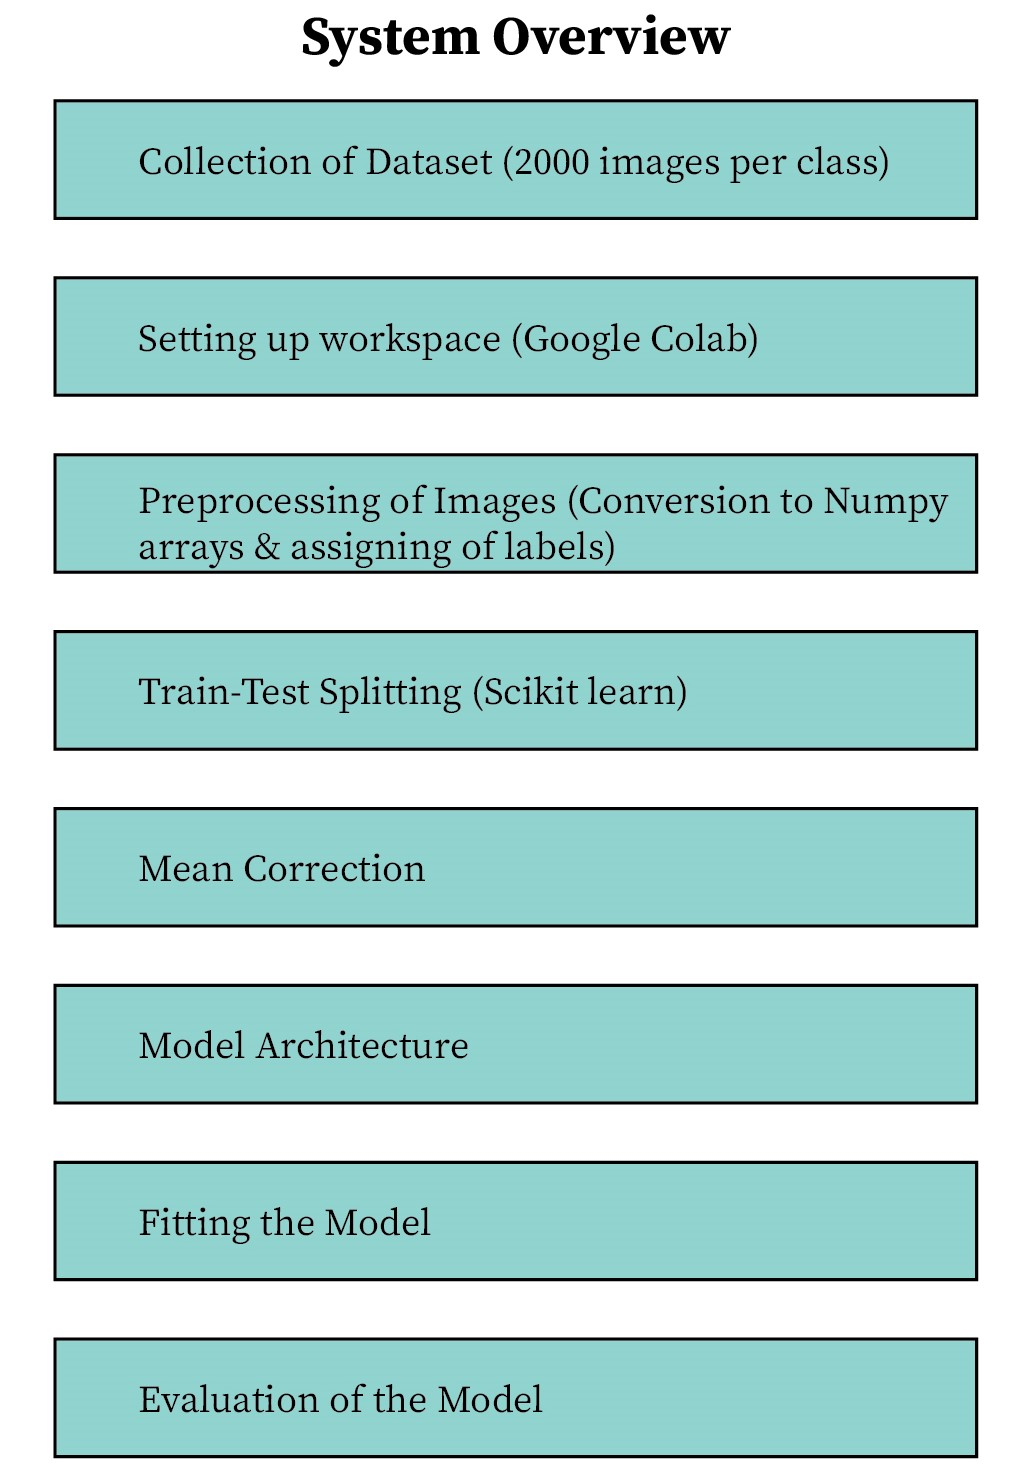
\includegraphics[scale = 0.9]{CHAPTERS/Chapter-4/Images/system_overview-01.jpg}
    \caption{System overview for a multi-class vehicles classifier  } 
    \label{system_overview}
  \end{figure}
\section{Formation of Dataset}
Deep learning based image classification works by inputting class
image examples to a CNN; CNN is then trained for higher test accuracy
and reduced test loss. The set of images used for this purpose is
called a dataset.
The dataset is divided into training and test dataset by a specific ratio.
In this project we have five different classes of vehicles i.e. Bus, Car, Truck, Motorcycle
and Hiace. There are a total of 10000 images with 2000 images of each 
class. These images are downloaded from Google search results and from already available
datasets and from websites providing licensed free images like Flickr.
APIs along with Python
scripts can be used to download these images from the internet.
Using matplotlib in python, we can plot some of the images with the output as
shown in listing \ref{listing:4.1} and plot is attached in figure
\ref{fig:4.1}.
\linespread{1.0}
\begin{listing}[H]
\begin{minted}[bgcolor=bg,
    linenos = true,
    xleftmargin=20pt,
    framesep = 2mm]{python}
import matplotlib.pyplot as plt
from matplotlib.image import imread  
path  = './images/'
for i in range(9):
    plt.subplot(330+1+i)
    filename = path + 'image_'+ str(i) + '.jpg'
    image = imread(filename)
    plt.imshow(image)    
    plt.show()
\end{minted}
\caption{Python script to plot some images from each class}
\label{listing:4.1}
\end{listing}

\begin{figure}[H]
    \centering
    \captionsetup{justification = centering}
    \includegraphics[scale = 0.8]{CHAPTERS/Chapter-4/Images/4.1.png}
    \caption{Plot of some images from each class} 
    \label{fig:4.1}
  \end{figure}

\subsection{Data Augmentation}
Training deep learning CNN architectures on larger datasets
results in more skillful models and improved classification accuracy.
However, availability of large amount of  class-specific data is a challenge.
This problem of lack of sufficient data can be solved using
techniques which expand the size of available data by introducing
modifications and variations by performing image manipulation.
Dataaugmentation is the process of applying techniques like shifting, 
flipping, rotating and varying the brightness etc on images to
introduce variations in images. The Keras deep learning NN library uses
ImageDataGenerator
class to achieve image data augmentation and is used in our code.

\section{Setting of Workspace for the Project}
There are a lot of images to be processed. To process images, high end GPU is
needed. Due to unavailability of an Nvidia GPU on the system, we used Google Colab.
It is an online platform having high end GPUs free provided by Google for training
up to 12 hours. Enabling a GPU in the notebook settings can accelerate the process of
training.
\section{Designing and Training of DCNN for Multi-Class Classification}
In our project we have used Keras for designing, training and testing of 
DCCN architectures for our multi-class classification problem.
Keras is one of the leading high level API for neural networks. It contains
many modules such as layers, cost functions, activation functions, initialization
schemes and regularization schemes. This project uses Keras for training purposes.
\subsection{Conversion of Images and Labels to Numpy Arrays}
After importing all the necessary packages, we are all set to pre-process our data.
Recall to chapter 2, where we studied the basics of an image. In Keras, an image has two
representations i.e. (width, height, color\_channels) and (color\_channels, width, height).
First approach is called as ``channels first approach" and
the latter is called as ``channels last approach".
We will use the ``channels last approach".

First step is to read the images from the folder mounted from Google drive.
Labels are assigned to classes from 0 to 4. Keras load\_img() routine loads image
from the folder with given target size. Target size for this project is chosen as
$128 \times 128$. This means that both width and height has a size of 128 pixels.
There are 3 color channels for RGB images. Images are then converted to numpy arrays using
Keras img\_to\_array() method. Labels are stored as 0, 1, 2, 3, 4 based on the class of image (as data is renamed).
Figure \ref{fig:class_labels} shows all the classes and corresponding labels.

\begin{figure}[H]
    \centering
    \captionsetup{justification = centering}
    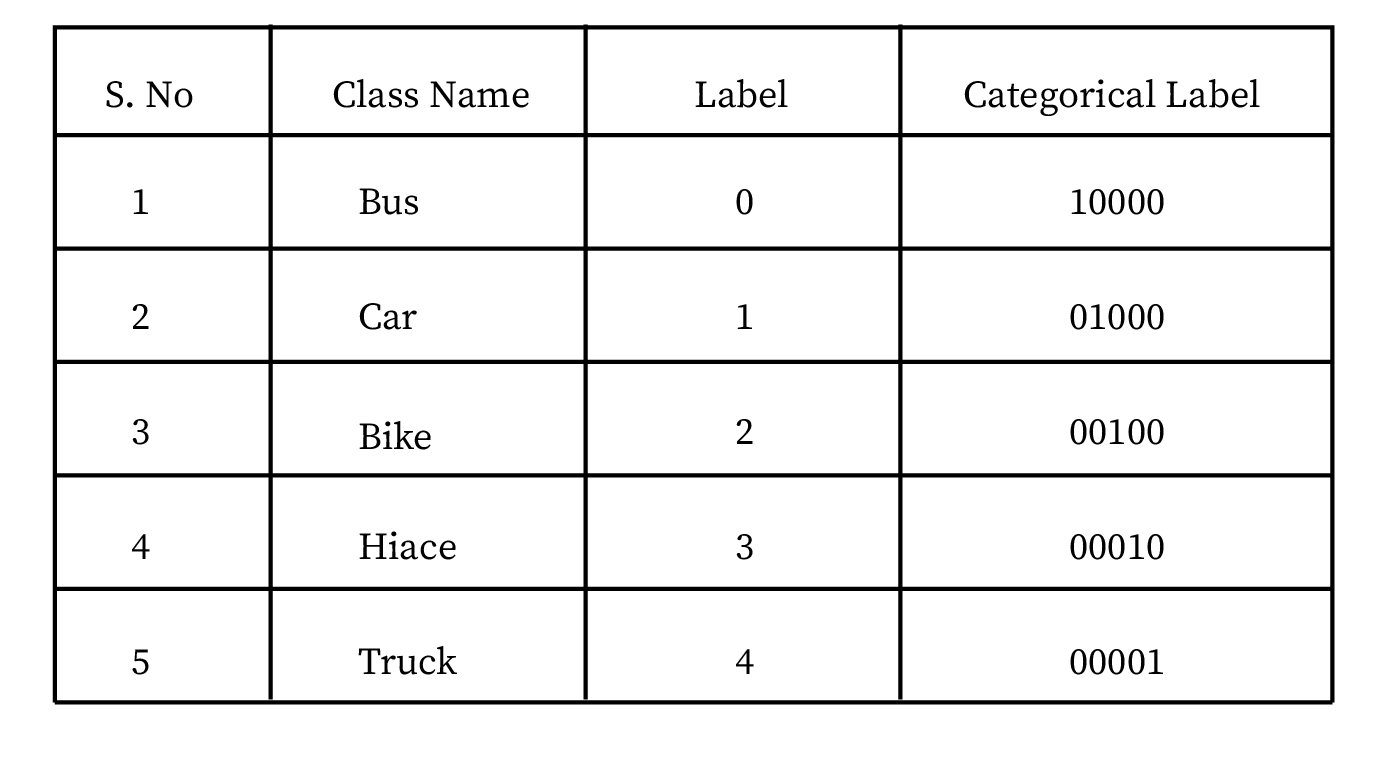
\includegraphics[scale = 0.2]{CHAPTERS/Chapter-4/Images/class_label-01}
    \caption{Classes and labels} 
    \label{fig:class_labels}
  \end{figure}

\noindent A section of code for this implementation is shown in listing \ref{listing:4.2}.

\begin{longlisting}
    \begin{minted}[bgcolor=bg,
        linenos = true,
        xleftmargin = 20pt,
        framesep = 2mm]{python}
folder = '/content/Input_data/'
images = np.zeros((num_of_images,img_rows,img_cols,color_channels))
labels = np.zeros(num_of_images)
i = 0
# enumerate files in the directory
for file in os.listdir(folder):
# determine class
    if file.startswith('bus'):
        output = 0
    elif file.startswith('car'):
        output = 1
    elif file.startswith('bike'):
        output = 2
    elif file.startswith('hiace'):
        output = 3
    else:
        output = 4
    # load image
    img = load_img(folder + file, target_size=(img_rows,img_cols))
    # convert to numpy array
    img = img_to_array(img)
    # store
    images[i] = img
    labels[i] = output
    i = i+1
\end{minted}

\caption{Conversion of Images to Numpy arrays}
\label{listing:4.2}
\end{longlisting}
In the code listing above ``images" on line 23, is a 4D tensor with
dimensions (10000, 128, 128, 3) which means that there are 10000
images with each image having $128\times 128\times 3$ matrices i.e.
each image has height and width of 128 pixels and 3 RGB channels in a
3D concurrent space. Also ,in the code listing above,
``labels", on line 24, is a 1D tensor containing the labels
for all the 10000 images available in our dataset.
\subsection{Train-Test Division}
In order to proceed with our DCNN multi-class classification model,
we need to split our available dataset into two parts, namely test 
dataset and train dataset. Both datasets have to be mutually-exclusive.
The train dataset is used for training our designed CNN.
Training involves three steps; feed forward, back propagation and
updation of model parameters. Test dataset is used to evaluate the performance
of our trained model on unseen data. Testing is a single step process
comprising of feed-forward only and it results in a  class
prediction for the input image. We used a ratio of 75\% and
25\% for train and test datasets respectively. The package used for this purpose is the
Scikit-learn train\_test\_split. Listing \ref{listing:4.3} shows splitting of
data into train and test.

\begin{listing}[H]
    \begin{minted}[bgcolor=bg,
        frame = lines,
        framesep = 2mm]{python}
train_images, test_images, train_labels, test_labels = 
train_test_split(images, labels, test_size = 0.25, random_state = 42)
\end{minted}
\caption{Train-test split}
\label{listing:4.3}
\end{listing}
There is another technique for splitting of data. In this technique, we make two directories,
namely, train and test and we randomly divide the images into these directories and then
convert them into numpy array. We have first converted the images
into arrays, split them into train and test and then we can save them back into
directories by converting them into images from array using PIL from\_array
function.

\subsection{Mean Correction}
After converting to float 32 and normalizing by 255, we have to subtract mean pixel.
Listing \ref{listing:4.4} illustrates the mean correction.

\begin{listing}[H]
    \begin{minted}[bgcolor=bg,
        linenos = true,
        xleftmargin = 20pt,
        framesep = 2mm]{python}
train_images = train_images.astype('float32') / 255
test_images = test_images.astype('float32') / 255

if subtract_pixel_mean:
    x_train_mean = np.mean(train_images, axis=0)
    train_images -= x_train_mean
    test_images -= x_train_mean

train_labels = to_categorical(train_labels,num_classes)
test_labels = to_categorical(test_labels,num_classes)
    \end{minted}
    \caption{Mean correction}
\label{listing:4.4}
\end{listing}
\noindent Lines 9 \& 10 shows the categorical labeling for using labels fit for Keras.
\subsection{CNN Model Architecture for Multi-Class Classification}
Recall from chapter \ref{Chapter 3}, a CNN model consists of various layers including
conv2D, Activation, MaxPoooling2D, Flatten and Dense layer.
Block diagram of the model architecture is shown in Figure \ref{fig:model_summary_2}. 
\begin{figure}[H]
    \centering
    \captionsetup{justification = centering}
    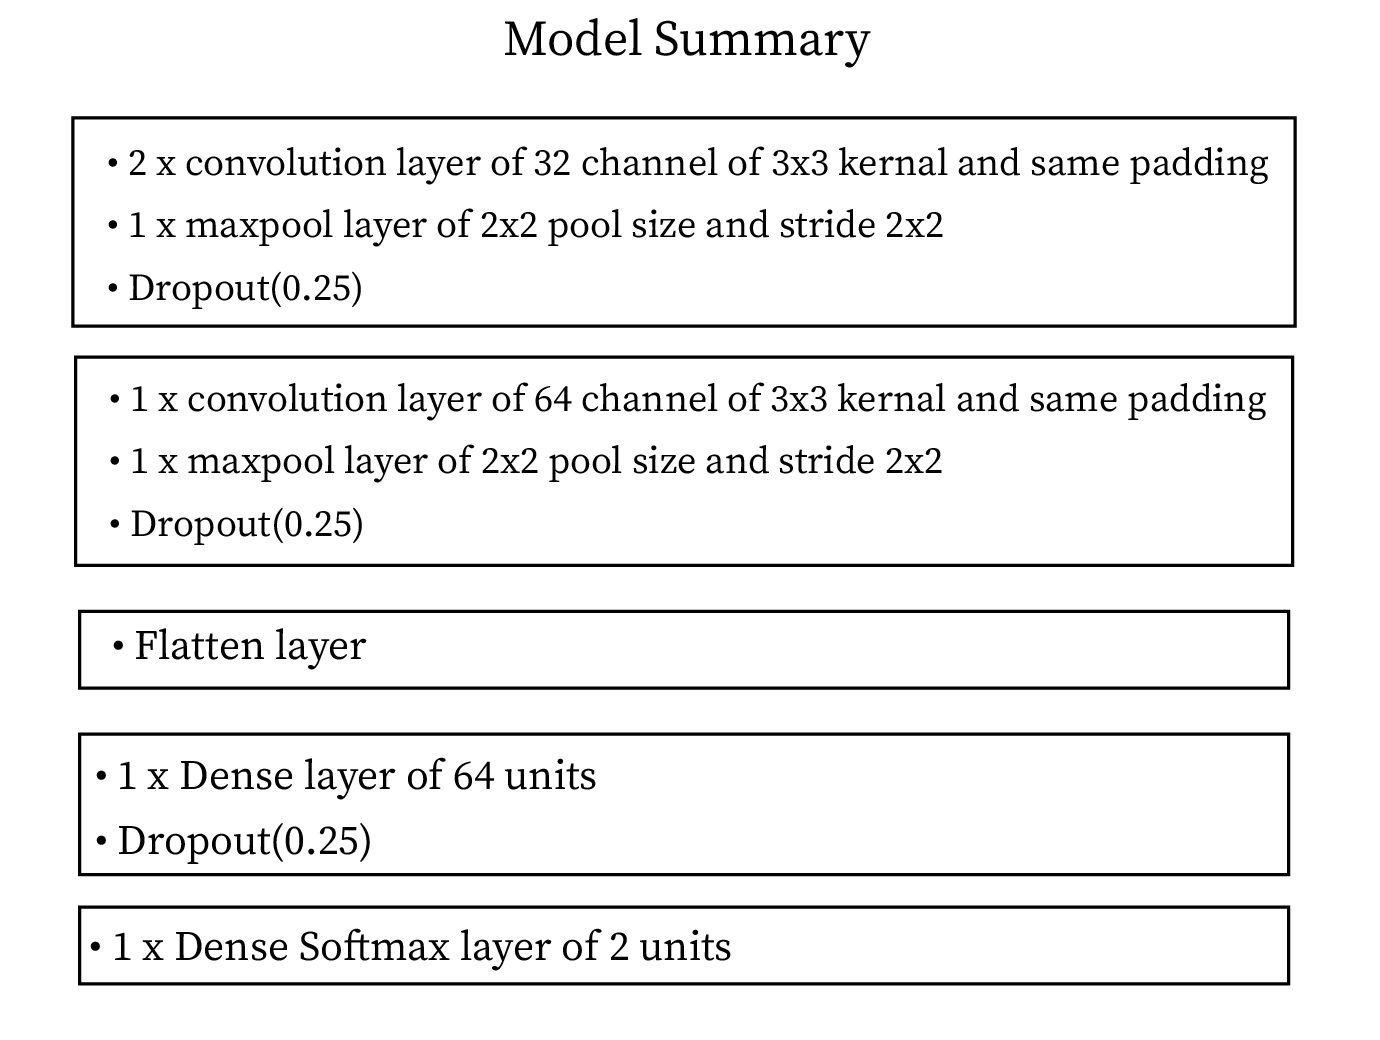
\includegraphics[scale = 1]{CHAPTERS/Chapter-4/Images/model_summary_2}
    \caption{Model architecture for binary class vehicle classifier} 
    \label{fig:model_summary_2}
\end{figure}
\noindent Listing \ref{listing:4.5}
defines the the architecture of our CNN Model.
\begin{longlisting}
    \begin{minted}[bgcolor=bg,
        linenos = true,
        xleftmargin = 20pt,
        framesep = 2mm]{python}
#Model
model = Sequential()
model.add(Conv2D(32, (3, 3), padding='same', activation = "relu",
                         input_shape=train_images.shape[1:]))
model.add(Conv2D(32, (3, 3), activation = "relu"))
model.add(MaxPooling2D(pool_size=(2, 2)))
model.add(Dropout(0.25))   

model.add(Conv2D(64, (3, 3), padding='same', activation = "relu"))
model.add(MaxPooling2D(pool_size=(2, 2)))
model.add(Dropout(0.25)) 
     
model.add(Flatten())

model.add(Dense(64))
model.add(Activation('relu'))
model.add(Dropout(0.5)) 

model.add(Dense(num_classes))
model.add(Activation('softmax'))

model.compile(loss='categorical_crossentropy', optimizer='adam',
metrics=['accuracy'])
    \end{minted}
    \caption{Defining the Model}
\label{listing:4.5}
\end{longlisting}
\noindent Lines 22 \& 23 define the loss function,
optimizer type and evaluation metrics used for training our CNN.
\subsubsection{Loss Function}

For more than two classes, loss is categorical\_crossentropy. For two
classes it is binary\_crossentropy. There are many optimizers in Keras i.e.
SGD, Adam, RMSprop, Adamax etc. Here we have used Adam. Accuracy metrics calculates how
often prediction equals labels.
\subsection{Fitting the Model}
Here the process of training starts. We have two functions used in Keras. One
is `model.fit' and other is `model.fit\_generator'. We have implemented data augmentation using a\
in our code using an if-else logic. We have also defined a validation set.
Validation data evalautes the behavior of the trained model to an unseen data.

An `epoch' is defined as a ``complete pass over an entire dataset" during the training process.
We have to determine the specific number of epochs for which the training process has to
run. If we pass over the entire dataset too many times,
it may result it increased training accuracy and reduced training loss
but it may also result in reduced validation accuracy and higher validation loss.
This specific scenario where validation accuracy is lower
than training accuracy or validation loss is higher  than
training loss is called ``overfitting''. Over-fitting means that our
CNN model has actually memorized the training examples or ``seen data"
instead of learning discernable parameters from it,
and it will not work well on `unseen data'. We have to avoid the overfitting. For this we have to search for
optimum values hyper-parameters of or model such as epochs,
batch size, optimizers, convolutional layers,
layer filters,filter sizes, drop-out layers etc.
Listing \ref{listing:4.6} shows the code for training process.

\begin{longlisting}
    \begin{minted}[bgcolor=bg,
        linenos = true,
        xleftmargin = 20pt,
        framesep = 2mm
        ]{python}
if not data_augmentation:
    print('Not using data augmentation.')
    history = model.fit(train_images, train_labels, validation_data =
    (test_images, test_labels), batch_size = batch_size, epochs = n_epochs)
else:
    datagen = ImageDataGenerator(
        zca_epsilon=1e-06,
        rotation_range=0,  
        width_shift_range=0.1,
        height_shift_range=0.1,
        shear_range=0.,
        zoom_range=0.,
        channel_shift_range=0.,
        fill_mode='nearest',
        cval=0.,
        rescale=None,
        preprocessing_function=None,
        data_format=None,
        validation_split=0.0)
    
    datagen.fit(train_images)
    
    history = model.fit_generator(datagen.flow(train_images, train_labels,
    batch_size = batch_size),validation_data=(test_images, test_labels),
    epochs = n_epochs)    
    \end{minted}
    \caption{Training the Model}
\label{listing:4.6}
\end{longlisting}
\subsection{Plotting the Accuracy and Loss}
A specific model with  chosen values of hyper-parameters
generates a specific accuracy upto which it can classify unseen data
Increasing epochs will not increase the accuracy, it basically overfits
the model. For a certain model, we have to find a specific number
of epochs. For this we plot the accuracy and loss of training and
validation data. Listing \ref{listing:4.7} shows the script for plotting the accuracy and
loss of training and validation data.

\begin{longlisting}
    \begin{minted}[bgcolor=bg,
        linenos = true,
        xleftmargin = 20pt,
        framesep = 2mm
        ]{python}
plt.grid()
plt.plot(history.history['accuracy'])
plt.plot(history.history['val_accuracy'])
plt.title('model accuracy')
plt.ylabel('accuracy')
plt.xlabel('epoch')
plt.legend(['train', 'validation'], loc='upper left')
plt.show()
# summarize history for loss
plt.grid()
plt.plot(history.history['loss'])
plt.plot(history.history['val_loss'])
plt.title('model loss')
plt.ylabel('loss')
plt.xlabel('epoch')
plt.legend(['train', 'val'], loc='upper left')
plt.show()
\end{minted}
\caption{Training, validation accuracy \& loss vs. epochs}
\label{listing:4.7}
\end{longlisting}

\subsection{Saving Model \& Weights}
After successful training of model, we have to resuse it
at evaluation or testing time. For this, the trained model is saved to our disk.
At testing time, this model can be loaded into Keras 
from our workspace. The Model is stored as .h5 file in the root directory.
Listing \ref{listing:4.8} shows the script for saving the weights.

\begin{listing}[H]
    \begin{minted}[bgcolor=bg,
        linenos = true,
        xleftmargin = 20pt,
        framesep = 2mm
        ]{python}
# Save model and weights
if not os.path.isdir(save_dir):
    os.makedirs(save_dir)
model_path = os.path.join(save_dir, model_name)
model.save(model_path)
print('Saved trained model at %s ' % model_path)
\end{minted}
\caption{Saving the Model}
\label{listing:4.8}
\end{listing}
\section{Evaluation of Model}
Evaluation of  the trained model over test dataset is  performed in two steps.
In the first step, the pre-trained model is loaded from the workspace.
In second step, `evaluate' function is used to run the run testing
phase on the test data. The function takes
test images and labels of the test images as input and, in turn,
generates a class label prediction for the input  test image. Listing \ref{listing:4.9} shows the script for
evalaution.
\begin{longlisting}
    \begin{minted}[bgcolor=bg,
        linenos = true,
        xleftmargin = 20pt,
        framesep = 2mm
        ]{python}
#Load Model
loaded_model = load_model("saved_models/model.h5")
#Evaluate Model
test_loss, test_acc = loaded_model.evaluate(test_images, test_labels)
print('Accuarcy of the model:', test_acc)
\end{minted}
\caption{Evaluating the Model}
\label{listing:4.9}
\end{longlisting}
\subsection{Two Class Problem \& Results}
We started with two class problem, Bus \& Car and recorded the results from 5
to 30 epochs.
The loss was binary\_crossentropy in this case. 
The training accuracy recorded after 25 epochs was 95.77\% and training
loss was 0.1269. The test set was choosen as validation data and validation accuracy after 5 epochs 
was 95.40\% and validation loss was 0.1271.
After 25 epochs for this model, the validation loss increases which indicate
that we have to train that model up to 20 epochs. The values of training
and validation accuracy \& training and validation loss
against number of epochs for binary class vehicle classifier
are tabulated in Table \ref{table:4.1}.
\begin{table}[H]
    \caption{Results for binary class vehicle classifier}
    \label{table:4.1}
	  \begin{center}
		\scalebox{0.85}
		{\begin{tabular}{|l |l |l |l |l |l |}
		\hline
		S.No & Number of epochs & Training accuracy & Validation accuracy & Training loss & Validation loss\\ \hline
		1  & 5 & 0.8783 & 0.9140 & 0.3083 & 0.2398
		\\ \hline
		2  & 10 & 0.9040 & 0.9440 & 0.2538 & 0.1585 
		\\ \hline
		3   & 15 & 0.9197  &  0.9410 & 0.2029 & 0.1652
        \\ \hline %
        4   & 20 &  0.9513 & 0.9650  &0.1408  & 0.0882
        \\ \hline %
        5   & 25 &  0.9577 & 0.9540  &0.1269  & 0.1271
        \\ \hline %
        6   & 30 &  0.9593 & 0.9550  &0.1126  & 0.1337
		\\ \hline %
		\end{tabular}}
	  \end{center}
\end{table}
\noindent The plot of training and validation accuracy and training and validation
losses for 30 epochs are plotted using Python matplotlib shown in figure \ref{fig:4.4}.
\begin{figure}[htbp]
    \centering
    \begin{subfigure}[t]{0.45\textwidth}
        \fbox{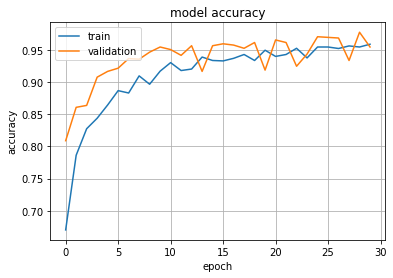
\includegraphics[scale = 0.5]{CHAPTERS/Chapter-4/Images/4.4a}}
        \caption{Training \& validation accuracy}
        \label{fig:4.4a}
    \end{subfigure}
    \begin{subfigure}[t]{0.45\textwidth}
        \fbox{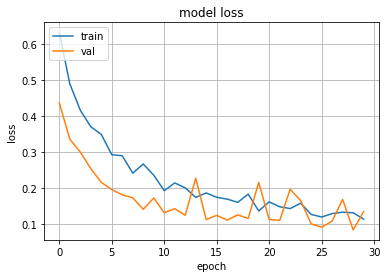
\includegraphics[scale = 0.5]{CHAPTERS/Chapter-4/Images/4.4b}}
        \caption{Training \& validation loss}
        \label{fig:4.4b}
    \end{subfigure}
    \caption[]{Model accuracy \& model loss}
    \label{fig:4.4}
  \end{figure}


\subsection{Five Class Probem \& Results}
We started with two class problem and extended the model to five classes
which is our desired task. The loss function in this case is categorical\_crossentropy.
The model used for five class is a customized VGG-16. The details of the
model are shown in figure \ref{model_summary}.
\begin{figure}[H]
    \centering
    \captionsetup{justification = centering}
    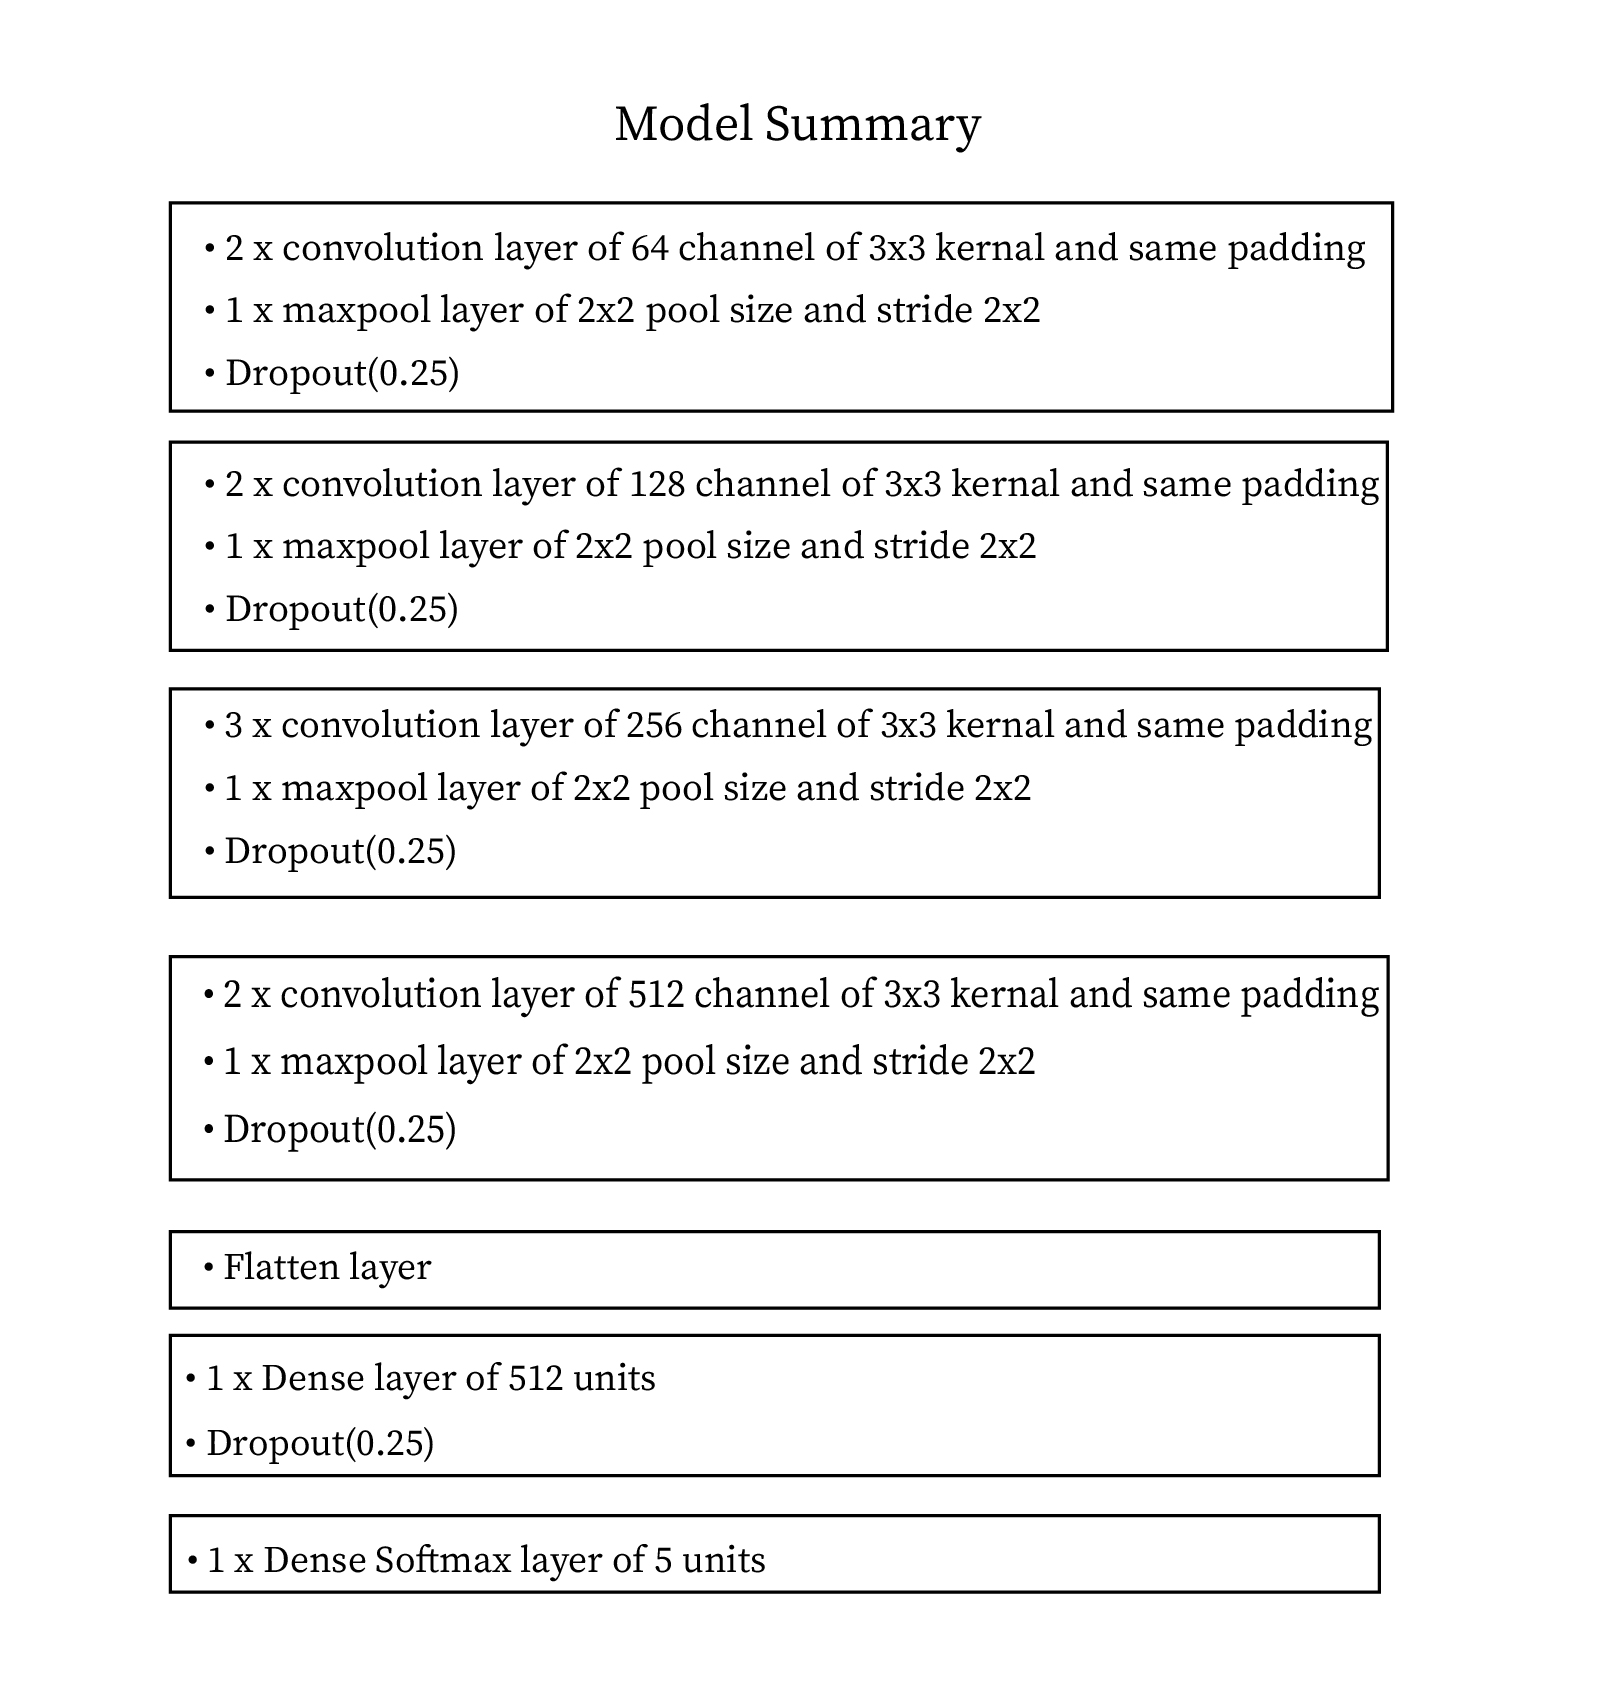
\includegraphics[scale = 0.8]{CHAPTERS/Chapter-4/Images/summary.jpg}
    \caption{Model architecture for five class vehicle classifier} 
    \label{model_summary}
\end{figure}
\noindent The optimizer used is RMSprop with
learning rate 0.0001. We started with 5 epochs, then 10 upto 20. The plot of training
and validation accuracy and training and validation loss is plotted using Python
matplotlib and it is observed that near to 20 the validation loss
increases and validation accuracy decreases. So we stopped at 20 epochs
and recorded the results. The plots are shown in
figure \ref{fig:4.6}.
\begin{figure}[htbp]
    \centering
    \begin{subfigure}[t]{0.45\textwidth}
        \fbox{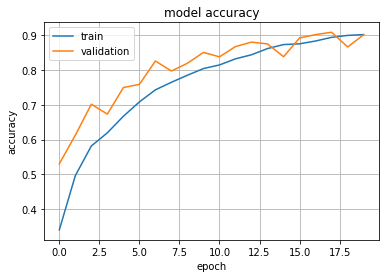
\includegraphics[scale = 0.5]{CHAPTERS/Chapter-4/Images/4.6a}}
        \caption{Training \& validation accuracy}
        \label{fig:4.4a}
    \end{subfigure}
    \begin{subfigure}[t]{0.45\textwidth}
        \fbox{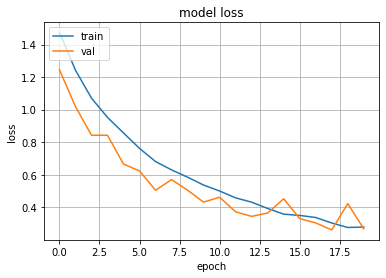
\includegraphics[scale = 0.5]{CHAPTERS/Chapter-4/Images/4.6b}}
        \caption{Training \& validation loss}
        \label{fig:4.4b}
    \end{subfigure}
    \caption[]{Model accuracy \& model loss}
    \label{fig:4.6}
  \end{figure}
  The loss was categorical\_crossentropy in this case. 
  The training accuracy recorded after 20 epochs was 90.2\% and training
  loss was 0.2778. The test set was choosen as validation data and
  validation accuracy after 20 epochs 
  was 90.16\% and validation loss was 0.2675.
  The values of training
  and validation accuracy \& training and validation loss
  against number of epochs for five class vehicle classifier
  are tabulated in Table \ref{table:4.2}.

\begin{table}[H]
    \caption{Results for binary class vehicle classifier}
    \label{table:4.2}
	  \begin{center}
		\scalebox{0.85}
		{\begin{tabular}{|l |l |l |l |l |l |}
		\hline
		S.No & Number of epochs & Training accuracy & Validation accuracy & Training loss & Validation loss\\ \hline
		1  & 5 & 0.6689 & 0.7644 & 0.8381 & 0.6587
		\\ \hline
		2  & 10 & 0.8253 & 0.8680 & 0.4851 & 0.3689
        \\ \hline %
        3   & 15 &  0.8741 & 0.8928  &0.3639  & 0.3084
        \\ \hline %
        4   & 20 &  0.9020 & 0.9016  &0.2778  & 0.2675
        \\ \hline %
		\end{tabular}}
	  \end{center}
\end{table}

\section{Graphical User Interface}
In order to observe the results visually we have developed a Graphical User
Interface (GUI) using tkinter package of 
Python. The test images are given as inputs to our trained
model one-by-one and corresponding labels are generated.
Since we cannot run tkinter on Google Colab,
so we saved our trained model in the local disk of our computer.
To visually display the testing results, all the images in the test dataset are used as inputs to the trained model that we have loaded  from our workspace
and the predicted class labels are displayed on the GUI accordingly.
Some examples are shown in
figure \ref{fig:4.7}.

\begin{figure}[htbp]
    \centering
    \begin{subfigure}[t]{0.3\textwidth}
        \fbox{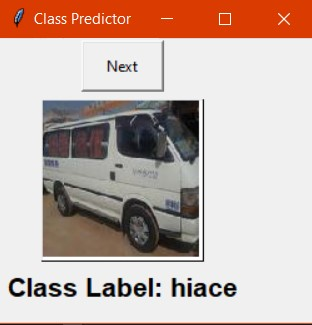
\includegraphics[width = 4.5cm, height = 4.5cm]{CHAPTERS/Chapter-4/Images/4.7a}}
        \caption{}
        \label{fig:4.7a}
    \end{subfigure}
    \begin{subfigure}[t]{0.3\textwidth}
        \fbox{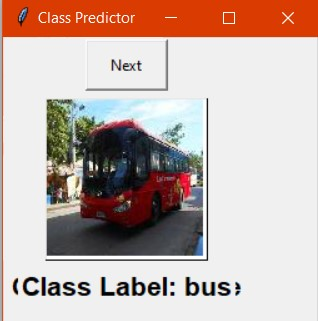
\includegraphics[width = 4.5cm, height = 4.5cm]{CHAPTERS/Chapter-4/Images/4.7b}}
        \caption{}
        \label{fig:4.7b}
    \end{subfigure}
    \begin{subfigure}[t]{0.3\textwidth}
      \fbox{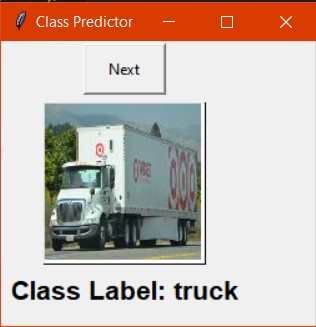
\includegraphics[width = 4.5cm, height = 4.5cm]{CHAPTERS/Chapter-4/Images/4.7c}}
      \caption{}
      \label{fig:4.7c}
  \end{subfigure}
    \captionsetup{justification = centering}
    \caption[]{Test images and labels on a GUI}
    \label{fig:4.7}
  \end{figure}

\section{Limitations \& Future Work}

For binary classification problem, the proposed model does not work on high resolution images.
Processing high resolution imagery might be a requirement in biomedical imaging,
since changing resolution might change the
local and global parameters content in the image. For high resolution images, we use Res-Net architecture which is complex and
requires high computational power. We have used a variant of VGG-16 for
our five class problem. Highly complex model may cause overfitting.
For future work, the detailed study
about tuning of hyperparameters is included.
Problem of overfitting can be eliminated by performing an
extensive search over hyper-parameters space to obtain optimum 
values of these parameters for our model.
Hyper-parameters include, no of convolutional layers, layer filters,
filter depth, pooling type, activation functions, length and number
of dense layers, drop-outs, batch-size,epochs, optimizers and loss
functions etc.

\addappheadtotoc
%\appendixpage
% \begin{appendices}
% \include{back/appendices/appendixA}
% \include{back/appendices/appendixB}
% \end{appendices}
% include your .bib file

\renewcommand{\bibname}{References}
\cleardoublepage
\phantomsection
\addcontentsline{toc}{chapter}{References}

\bibliography{thesis}
\bibliographystyle{IEEEtr}
%\include{back/about_the_author/about_the_author}
\end{document}
